\documentclass[a4paper,oneside,12pt]{article}
\usepackage{graphics,multicol}
\usepackage[latin1]{inputenc}
\usepackage[a4paper,margin=2cm,lmargin=2cm,headheight=1pt]{geometry}
\usepackage{fancyhdr}
\usepackage{amsmath,amssymb,amsfonts,amsthm, mathrsfs}
\usepackage{mathtools,bbm}
\usepackage{IEEEtrantools}
\usepackage[]{algorithm2e}
\usepackage{tikz,pgfplots,tkz-graph}
\usepackage{ifthen,calc}
\usepackage{listings,hyperref,float}
\usepackage{epsfig,epstopdf,graphicx}
\usepackage{enumerate}

\pgfplotsset{compat=newest}
\usetikzlibrary{positioning,matrix}
\interdisplaylinepenalty=2500

% Page settings
% \setlength{\oddsidemargin}{0 in}
% \setlength{\evensidemargin}{0 in}
% \setlength{\topmargin}{-0.6 in}
% \setlength{\textwidth}{6.5 in}
% \setlength{\textheight}{8.5 in}
% \setlength{\headsep}{0.75 in}
% \setlength{\parindent}{0 in}
% \setlength{\parskip}{0.1 in}

% Markov symbol X -o- Y
\newcommand{\markov}{\mathrel{\multimap}\joinrel\mathrel{-}\joinrel\mathrel{\mkern-6mu}\joinrel\mathrel{-}}
% Independent & not independent symbol X _||_ Y
\newcommand{\indep}{\mathrel{\bot}\joinrel\mathrel{\mkern-5mu}\joinrel\mathrel{\bot}}
\newcommand{\dep}{\centernot\indep}
% i.i.d.
\newcommand{\iid}{\stackrel{\mathrm{i.i.d.}}{\sim}}
% Integration d
\newcommand{\dd}{\mathop{}\!\mathrm{d}}

% Single braces
\newcommand{\agbrs}[1]{\left\langle #1 \right\rangle}	% angle braces,  	< x >
\newcommand{\rdbrs}[1]{\left( #1 \right)}				% round braces,  	( x )
\newcommand{\sqbrs}[1]{\left\lbrack #1 \right\rbrack}	% square braces, 	[ x ]
\newcommand{\clbrs}[1]{\left\lbrace #1 \right\rbrace}	% curly braces, 	{ x }

% Delimited braces
\newcommand{\agbrsv}[2]{\left\lange #1 \,\middle|\, #2 \right\rangle}	% angle braces with delimiter |,  	< x | y >, inner product
\newcommand{\rdbrsv}[2]{\left( #1 \,\middle|\, #2 \right)}				% round braces with delimiter |,  	( x | y ), conditional probability
\newcommand{\sqbrsv}[2]{\left\lbrack #1 \,\middle|\, #2 \right\rbrack}	% square braces with delimiter |,  	[ x | y ], conditional expectation
\newcommand{\clbrsv}[2]{\left\lbrace #1 \,\middle|\, #2 \right\rbrace}	% curly braces with delimiter |,  	{ x | y }, set

% Short for underline and overline
\newcommand{\udl}[1]{\underline{#1}}
\newcommand{\ovl}[1]{\overline{#1}}

% Derivative and partial derivation
\newcommand{\fracd}[2]{ \frac{\mathrm{d} #1}{\mathrm{d} #2} }
\newcommand{\fracp}[2]{ \frac{\partial #1}{\partial #2} }

% Absolute value, norm, ceil, floor, and evaluation
\newcommand{\abs}[1]{\left| #1 \right|}		% Absolute value, 	| x |
\newcommand{\norm}[1]{\left\| #1 \right\|}	% Norm, 			|| x ||
\DeclarePairedDelimiter\ceil{\lceil}{\rceil}
\DeclarePairedDelimiter\floor{\lfloor}{\rfloor}
\newcommand{\eval}[1]{\left. #1 \right|}	% Evaluation, 		f(x) |_{x=x0}

% Definition equal sign
\newcommand{\defeq}{\vcentcolon=}   % :=
\newcommand{\eqdef}{=\vcentcolon}   % =:
\newcommand{\texteq}[1]{\stackrel{#1}{=\joinrel=\joinrel=}}   % use for change of variable

% Inverse hyperbolic functions
\DeclareMathOperator\arcsinh{arcsinh}
\DeclareMathOperator\arccosh{arccosh}
\DeclareMathOperator\arctanh{arctanh}
\DeclareMathOperator\atanh{atanh}
\DeclareMathOperator\sech{sech}

% argmax and argmin
\newcommand\limit[1]{\underset{#1}{\lim}\,}
\newcommand\argmax[1]{\mathrm{arg}\,\underset{#1}{\max}\,}
\newcommand\argmin[1]{\mathrm{arg}\,\underset{#1}{\min}\,}

% Matrices
\newcommand*\pmtx[1]{\begin{pmatrix}#1\end{pmatrix}}			% Matrix with round braces
\newcommand*\bmtx[1]{\begin{bmatrix}#1\end{bmatrix}}			% Matrix with square braces
\newcommand*\vmtx[1]{\begin{vmatrix}#1\end{vmatrix}}			% Determinant of matrix
\newcommand*\spmtx[1]{\rdbrs{\begin{smallmatrix}#1\end{smallmatrix}}}	% Small matrix with round braces
\newcommand*\sbmtx[1]{\sqbrs{\begin{smallmatrix}#1\end{smallmatrix}}}	% Small matrix with square braces
\newcommand*\svmtx[1]{\abs{\begin{smallmatrix}#1\end{smallmatrix}}}		% Determinant of small matrix
\newcommand{\sizecorr}[1]{\makebox[0cm]{\phantom{$\displaystyle #1$}}}	% Get size of an expression

% Theorem environments
\newtheorem{theorem}{Theorem}
\newtheorem{corollary}[theorem]{Corollary}
\newtheorem{lemma}[theorem]{Lemma}
\newtheorem{observation}[theorem]{Observation}
\newtheorem{proposition}[theorem]{Proposition}
\newtheorem{definition}[theorem]{Definition}
\newtheorem{claim}[theorem]{Claim}
\newtheorem{fact}[theorem]{Fact}
\newtheorem{assumption}[theorem]{Assumption}

\newtheorem*{theorem*}{Theorem}
\newtheorem*{corollary*}{Corollary}
\newtheorem*{lemma*}{Lemma}
\newtheorem*{proposition*}{Proposition}
\newtheorem*{definition*}{Definition}
\newtheorem*{example*}{Example}
\newtheorem*{remark*}{Remark}
\newtheorem*{problem*}{Problem}

% Solution environment
\newenvironment{solution}{\begin{proof}[Solution]}{\end{proof}}

% Short for boldsymbol
\newcommand{\bs}[1]{\boldsymbol{#1}}

% Other frequent used operators
\def\Var{\mathsf{Var}}
\def\Cov{\mathsf{Cov}}
\def\coeff{\mathsf{coeff}}
\def\Tr{\mathsf{Tr}}
\def\rank{\mathsf{rank}}
\def\diag{\mathsf{diag}}
\def\mse{\mathsf{mse}}
\def\mmse{\mathsf{mmse}}

\def\ee{\mathbbm{e}}
\def\ii{\mathbbm{i}}
\def\EE{\mathsf{E}}
\def\FF{\mathsf{F}}
\def\SS{\mathsf{S}}
\def\UU{\mathsf{U}}
\def\xx{\mathsf{x}}
\def\pprime{{\prime\prime}}

\newcommand{\KL}[2]{D\left( #1 \,\middle|\middle|\, #2 \right)}%                   ( | )

\makeatletter
\newcommand\ztag[1]{%
\def\@currentlabel{#1}%
\gdef\tmp{%
\addtocounter{equation}{-1}%
\def\theequation{#1}}%
\aftergroup\aftergroup\aftergroup\aftergroup\aftergroup\aftergroup
\aftergroup\aftergroup\aftergroup\aftergroup\aftergroup\aftergroup
\aftergroup\aftergroup\aftergroup\aftergroup\aftergroup\aftergroup
\aftergroup\aftergroup\aftergroup\aftergroup\aftergroup\aftergroup
\aftergroup\aftergroup\aftergroup\aftergroup\aftergroup\aftergroup
\aftergroup
\tmp\IEEEyesnumber}


\pagestyle{empty}
\begin{document}

\noindent

\begin{tabular}{lcr}
  Duke University & & Math 690-40 \\  
  Homework two & \hspace{6.3cm} & F. Krzakala and L. Zdeborov\'a\\ \hline
\end{tabular}

\begin{center}
  {\Large {\bf p-spin model and belief propagation}}
\end{center}

%\subsection*{Representing problems by graphical models}



\subsection*{1. The ``$ 3 $-spin'' Curie-Weiss model}
The 3-spin ferromagnetic model is a generalization of the Curie-Weiss model that reads
\begin{equation*}
    \mathcal{H} \rdbrs{ \clbrs{ S_i }_{i=1}^N } = -\frac{1}{N^2} \sum_{i,j,k} S_i S_j S_k - h \sum_i S_i
    = -N \sqbrs{ \rdbrs{ \frac{\sum_i S_i}{N} }^3 + h \frac{\sum_i S_i}{N} }
\end{equation*}

\begin{enumerate}[(a)]
\item 
        Using the method we developed in the lecture, by computing the number of configuration with a given magnetization $ m $ and then using the Stirling formula, show that the free energy per spin of the 3-spin model 
        $
            f(\beta, h) = -\frac{1}{N \beta} \limit{N \to \infty} \log{Z_N(\beta,h)}
        $
        can be written (asymptotically) as
        $
            f(\beta, h) = \min_{m \in [-1,1]} \mathcal{F}_m(\beta, h, m)
        $,
        with the free energy at fixed magnetization $ \mathcal{F}_m(\beta, h, m) $ being given by:
        \begin{equation*}
            \mathcal{F}_m(\beta, h, m)
            = -m^3 - h m + \frac{1}{\beta} \sqbrs{ \frac{1+m}{2} \log \rdbrs{ \frac{1+m}{2} } + \frac{1-m}{2} \log \rdbrs{ \frac{1-m}{2} } }
        \end{equation*}
        and the equilibrium value of the magnetization is given by the minimizer $ m^* $:
        \begin{equation*}
            \agbrs{ \frac{\sum_i S_i}{N} } = m^*
        \end{equation*}
\item 
        Consider the case $ h=0 $ (also in part (c) and (d)) and plot the function $ \mathcal{F}_m(\beta, h=0, m) $ as a function of $ m $ for different values of the inverse temperature $ \beta $.
        Compute the value of $ m^* $ for many temperatures to show that it has a \textit{first order transition} (that is: there is a discontinuity).
\item 
        Show (numerically) that there is are three regions: for $ \beta < \beta_{\mathrm{s}} $ there is a unique minima in $ m=0 $. 
        For $ \beta_{\mathrm{s}} < \beta < \beta_{\mathrm{c}} $ a second local minima appears. 
        For $ \beta_{\mathrm{c}} < \beta $ the second minima is now the global one. 
        Find the values of $ \beta_{\mathrm{s}} $ and $ \beta_{\mathrm{c}} $.
% \item 
%         \textbf{BONUS}: using the method that we have seen in the third lecture, using the $ \delta $ and its Fourier transform, show that the free energy can also be written as
%         \begin{equation*}
%             \min_{m \in [-1,1]} \sqbrs{ 2 m^3 - \frac{1}{\beta} \log \sqbrs{ 2 \cosh \rdbrs{ 3 \beta m^2 + \beta h } } }
%         \end{equation*}
\item
        Describe your expectation about the long-time (but not exponentially in $ N $ long) behavior of the Monte Carlo Markov Chain designed to sample the Boltzmann distribution. 
        When initialized at magnetization $ m=0 $, and when initialized at $ m=1 $. 
        You can modify your code from the previous homework to support your intuition.
\end{enumerate}
\begin{solution} $\,$ 
\begin{enumerate}[(a)]
\item 
        First for notation simplicity, define the natural-based entropy function
        \begin{equation*}
            H_{\ee}(x) = -x \log(x) - (1-x) \log(1-x)
        \end{equation*}
        Denote $ \mathcal{N}(m) $ to be the number of configurations with magnetization $ m $, it is easy to see
        \begin{IEEEeqnarray*}{rCl}
            \mathcal{N}(m)
            &=& \binom{ N }{ \frac{N+Nm}{2} }
            = \frac{ N! }{ \rdbrs{ \frac{1+m}{2} N }! \rdbrs{ \frac{1-m}{2} N }! }
        \end{IEEEeqnarray*}
        When $ N \to \infty $, use Stirling formula
        \begin{IEEEeqnarray*}{rCl}
            \mathcal{N}(m)
            &\approx& \frac{ \sqrt{ 2 \pi N } \rdbrs{ \frac{N}{\ee} }^N }{ \sqrt{ 2 \pi \frac{1+m}{2} N } \rdbrs{ \frac{(1+m)N}{2\ee} }^{\frac{1+m}{2}N} \cdot \sqrt{ 2 \pi \frac{1-m}{2} N } \rdbrs{ \frac{(1-m)N}{2\ee} }^{\frac{1-m}{2}N} } \\
            &=& \sqrt{ \frac{2}{ (1-m^2) \pi N } } \exp \rdbrs{ -N \sqbrs{ \frac{1+m}{2} \log \rdbrs{ \frac{1+m}{2} } + \frac{1-m}{2} \log \rdbrs{ \frac{1-m}{2} } } } \\
            &=& \exp \rdbrs{ -N \sqbrs{ \frac{1+m}{2} \log \rdbrs{ \frac{1+m}{2} } + \frac{1-m}{2} \log \rdbrs{ \frac{1-m}{2} } + \mathrm{o}(1) } } \\
            &=& \exp \rdbrs{ N \sqbrs{ H_{\ee} \rdbrs{ \frac{1+m}{2} } + \mathrm{o}(1) } } \IEEEyesnumber \label{eq:A_a_Nm}
        \end{IEEEeqnarray*}
        Given the Hamiltonian $ \mathcal{H} $, we can write down the partition function
        \begin{IEEEeqnarray*}{rCl}
            Z_N(\beta, h)
            &=& \sum_{ \clbrs{ S_i }_{i=1}^N } \exp \rdbrs{ -\beta \mathcal{H} \rdbrs{ \clbrs{ S_i }_{i=1}^N } } \\
            &=& \sum_{ \clbrs{ S_i }_{i=1}^N } \exp \rdbrs{ N \beta \sqbrs{ \rdbrs{ \frac{\sum_i S_i}{N} }^3 + h \frac{\sum_i S_i}{N} } } \\
            &=& \sum_{ \substack{m = -1 \\ \text{step } \frac{2}{N} }}^{+1} \sum_{ \clbrs{ S_i }_{i=1}^N } \mathbb{I} \rdbrs{ \frac{\sum_i S_i}{N} = m } \exp \rdbrs{ N \beta \sqbrs{ \rdbrs{ \frac{\sum_i S_i}{N} }^3 + h \frac{\sum_i S_i}{N} } } \\
            &=& \sum_{ \substack{m = -1 \\ \text{step } \frac{2}{N} }}^{+1} \mathcal{N}(m) \exp \rdbrs{ N \beta \rdbrs{ m^3 + h m } } \IEEEyesnumber \label{eq:A_a_ZN}
        \end{IEEEeqnarray*}
        As $ N \to \infty $, by plugging eqn~\ref{eq:A_a_Nm} to eqn~\ref{eq:A_a_ZN} and notice that the $ \mathrm{o}(1) $ term is negligible, the free energy per spin can be computed as
        \begin{IEEEeqnarray*}{rCl}
            f(\beta, h)
            &=& -\limit{N \to \infty} \frac{1}{N \beta} \log \rdbrs{ Z_N(\beta, h) } \\
            &=& -\limit{N \to \infty} \frac{1}{N \beta} \log \clbrs{ \sum_{ \substack{m = -1 \\ \text{step } \frac{2}{N} }}^{+1} \mathcal{N}(m) \exp \rdbrs{ N \beta \rdbrs{ m^3 + h m } } } \\
            &=& -\limit{N \to \infty} \frac{1}{N \beta} \log \clbrs{ \int_{-1}^{+1} \dd m \, \exp \rdbrs{ N \beta \rdbrs{ m^3 + h m - \frac{1}{\beta} H_{\ee} \rdbrs{ \frac{1+m}{2} } + \mathrm{o}(1) } } } \\
            &\texteq{\text{Laplace}}& -\frac{1}{\beta} \max_{m \in [-1,1]} \sqbrs{ \beta \rdbrs{ m^3 + hm - \frac{1}{\beta} H_{\ee} \rdbrs{ \frac{1+m}{2} } } } \\
            &=& \min_{m \in [-1,1]} \sqbrs{ -m^3 - hm + \frac{1}{\beta} H_{\ee} \rdbrs{ \frac{1+m}{2} } } \\
            &=& \min_{m \in [-1,1]} \mathcal{F}_m(\beta, h, m)
        \end{IEEEeqnarray*}
        When $ N $ is large, the Boltzmann distribution is dominated by the `typical' configurations $ \clbrs{ S_i }_{i=1}^N $ such that $ \sum_i S_i / N = m^* $, where $ m^* $ is the minimizer of $ \mathcal{F}_m(\beta, h, m) $.
        Therefore, when we compute the Boltzmann average $ \agbrs{ \sum_i S_i / N } $, in the large $ N $ limit it is just the magnetization of `typical' configurations, which is $ m^* $.
\item 
        The plot of function $ \mathcal{F}_m(\beta, h, m) $ under $ h = 0 $ and $ \beta = 0.5, 0.578, 0.673, 1, 1.5, 2.5, 5 $, the local minima are marked at dot.
        \begin{figure}[H]
            \centering
            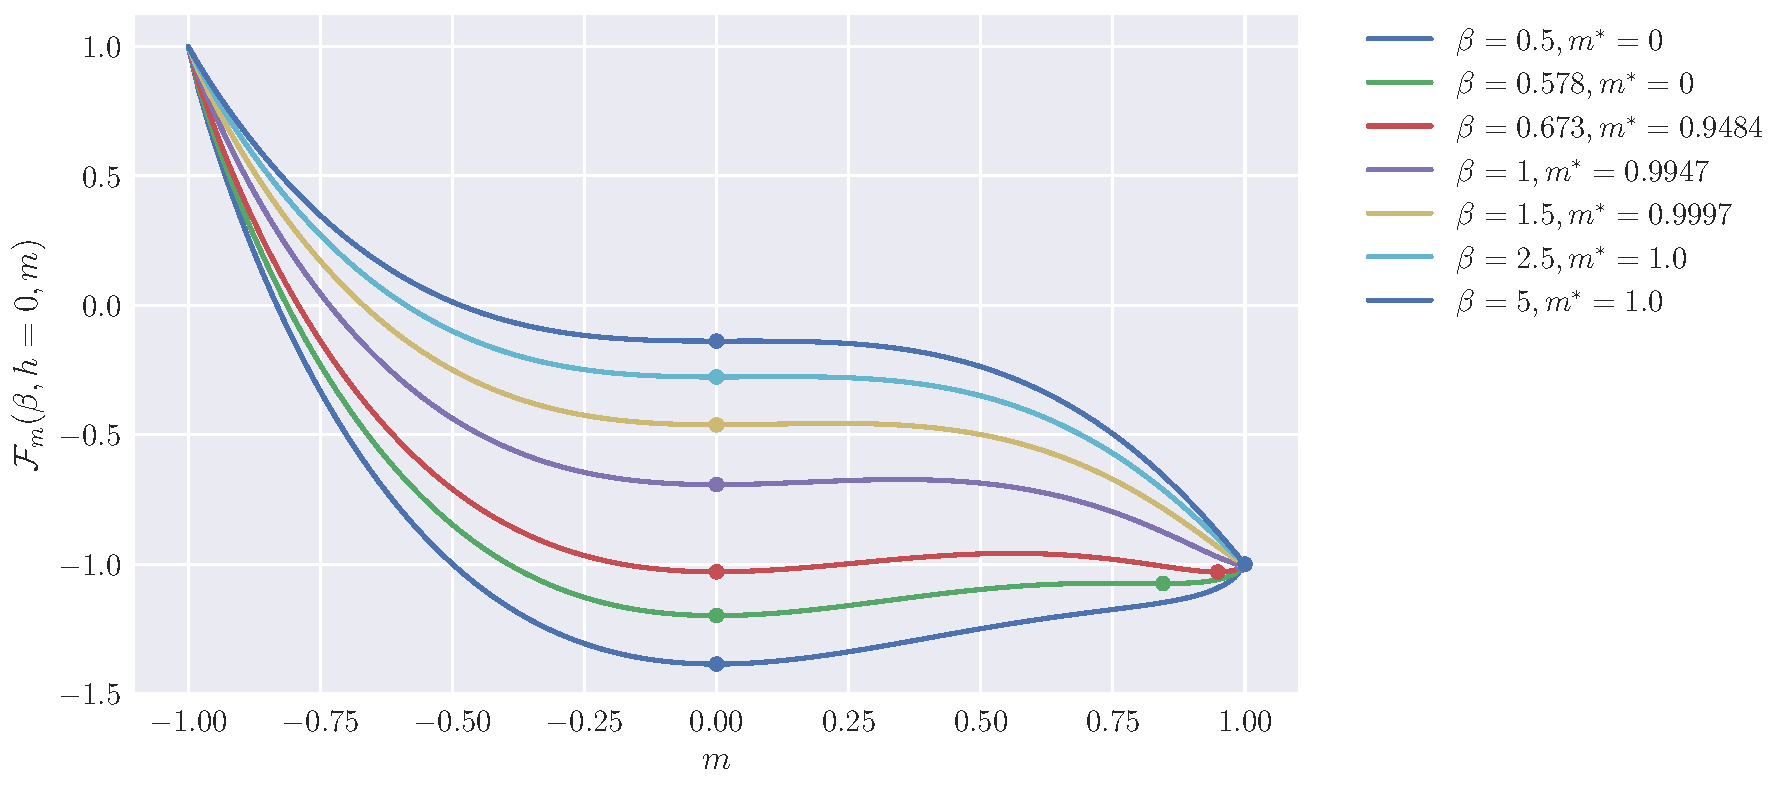
\includegraphics[width=450pt]{hw2/hw2_1(b).pdf}
        \end{figure}
        It can be seen when $ m = 0 $ is always a local minima, as $ \beta $ increases to some value, the second local minima emerges at right side but the global minima is still at $ m = 0 $.
        If $ \beta $ keeps on increasing to a higher value, the global minima suddenly jumps to the right local minima, causing a discontinuity on $ m^*(\beta, h) $.
\item   To prove $ m = 0 $ is always a local minima
        \begin{IEEEeqnarray*}{rCl}
            \eval{\fracp{}{m} \mathcal{F}_m(\beta, h, m)}_{\substack{h=0 \\ m=0}}
            &=& \eval{ -3 m^2 - h + \frac{\atanh(m)}{\beta} }_{\substack{h=0 \\ m=0}} = 0 \\
            \eval{\frac{\partial^2}{\partial m^2} \mathcal{F}_m(\beta, h, m)}_{\substack{h=0 \\ m=0}}
            &=& \eval{-6 m + \frac{1}{(1-m^2) \beta}}_{\substack{h=0 \\ m=0}}
            = \frac{1}{\beta} > 0
        \end{IEEEeqnarray*}
        Define the right-most local minima to be
        \begin{equation*}
            \tilde{m}(\beta, h) = \max \clbrsv{ m }{ \fracp{}{m} \mathcal{F}_m(\beta,h,m) = 0 }
        \end{equation*}
        The plot of $ m^*(\beta, h) $ and $ \tilde{m}(\beta, h) $ under $ h = 0 $ and $ \beta^{-1} \in (0,2] $ is
        \begin{figure}[H]
            \centering
            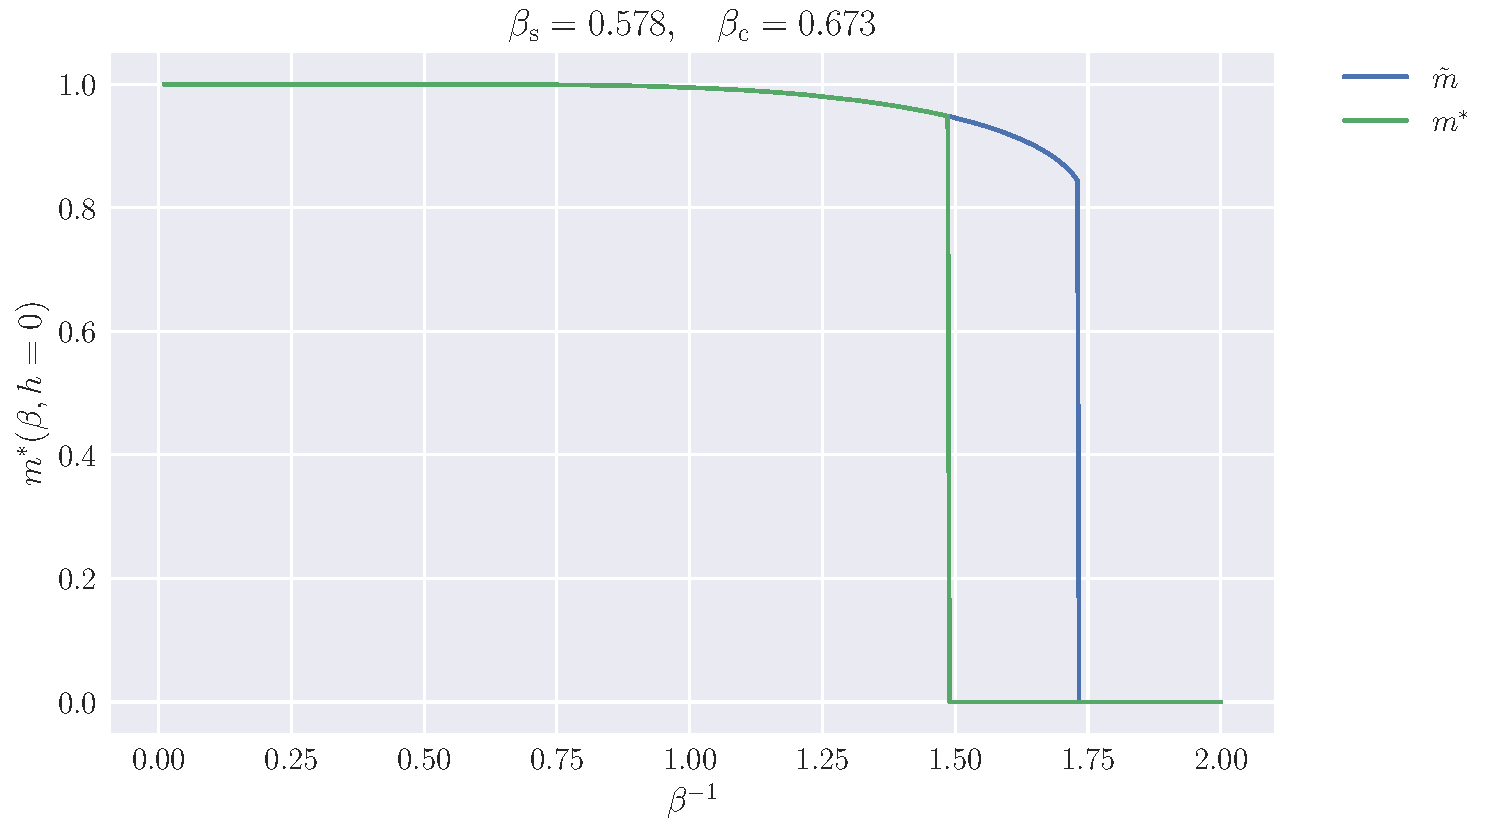
\includegraphics[width=370pt]{hw2/hw2_1(c).pdf}
        \end{figure}
        It is easy to see both curves have jumps, the second local minima emerges when the blue curve jumps, the second local minima becomes global minima when the green curve jumps.
\item 
        Using the $ \delta $ function and Fourier trick,

        \begin{IEEEeqnarray*}{rCl}
            Z_N(\beta, h)
            &=& \sum_{ \clbrs{ S_i }_{i=1}^N } \exp \rdbrs{ N \beta \sqbrs{ \rdbrs{ \frac{\sum_i S_i}{N} }^3 + h \frac{\sum_i S_i}{N} } } \\
            &=& \sum_{ \clbrs{ S_i }_{i=1}^N } \int \dd m \, \delta \rdbrs{ \frac{\sum_i S_i}{N}, m } \exp \rdbrs{ N \beta \rdbrs{ m^3 + hm } } \\
            &=& \sum_{ \clbrs{ S_i }_{i=1}^N } \int \dd m \, \int \dd \lambda \, \exp \rdbrs{ 2 \pi \ii \lambda \sqbrs{ N m - \sum_i S_i } } \exp \rdbrs{ N \beta \rdbrs{ m^3 + hm } } \\
            &\texteq{\hat{m} = 2\pi \ii \lambda}& \sum_{ \clbrs{ S_i }_{i=1}^N } \int_{\mathbb{R}} \dd m \int_{-2\pi\ii\infty}^{2\pi\ii\infty} \dd \hat{m} \, \exp \rdbrs{ \hat{m} \sqbrs{ N m - \sum_i S_i } } \exp \rdbrs{ N \beta (m^3 + h m) } \\
            &=& \int_{\mathbb{R}} \dd m \int_{-2\pi\ii\infty}^{2\pi\ii\infty} \dd \hat{m} \, \underbrace{ \sqbrs{ \sum_{ \clbrs{ S_i }_{i=1}^N } \exp \rdbrs{ -\hat{m} \sum_i S_i } } }_{= \sqbrs{ 2 \cosh(\hat{m}) }^N } \exp \rdbrs{ N \beta (m^3 + h m) + N \hat{m} m } \\
            &=& \iint \dd m \dd \hat{m} \exp \clbrs{ N \beta \sqbrs{ m^3 + h m + \frac{1}{\beta} \hat{m} m + \frac{1}{\beta} \log \rdbrs{ 2 \cosh(\hat{m}) } } }
        \end{IEEEeqnarray*}
        Apply the saddle-point method, take partial derivative w.r.t. $ \hat{m} $ gives
        \begin{IEEEeqnarray*}{rCl}
            0 &=& \fracp{}{m} \sqbrs{ m^3 + h m + \frac{1}{\beta} \hat{m} m + \frac{1}{\beta} \log \rdbrs{ 2 \cosh(\hat{m}) } }
            = 3 m^3 + h + \frac{1}{\beta} \hat{m} \\
            0 &=& \fracp{}{\hat{m}} \sqbrs{ m^3 + h m + \frac{1}{\beta} \hat{m} m + \frac{1}{\beta} \log \rdbrs{ 2 \cosh(\hat{m}) } }
            = \frac{1}{\beta} m + \frac{1}{\beta} \tanh(\hat{m}) \\
            \Rightarrow &&
            \begin{cases}
                m = -\tanh(\hat{m}) \\
                \hat{m} = -\beta \rdbrs{ 3 m^2 + h } \\
            \end{cases} \\
            f(\beta, h)
            &=& -\limit{N \to \infty} \frac{1}{N \beta} \log \rdbrs{ Z_N(\beta) } \\
            &\texteq{ \hat{m} = -\beta \rdbrs{ 3 m^2 + h } }& -\max_{m \in [-1,1]} \sqbrs{ -2 m^3 + \frac{1}{\beta} \log \sqbrs{ 2 \cosh \rdbrs{ 3 \beta m^2 + \beta h } } } \\
            &=& \min_{m \in [-1,1]} \sqbrs{ 2 m^3 - \frac{1}{\beta} \log \sqbrs{ 2 \cosh \rdbrs{ 3 \beta m^2 + \beta h } } }
        \end{IEEEeqnarray*}

\item   
        To describe the long-time (but not exponentially in $ N $ long) behavior of the Monte Carlo Markov Chain, we need to consider cases according to $ \beta $
        \begin{itemize}
        \item   $ \beta < \beta_{\mathrm{s}} $:
                There is only one local minima at $ m = 0 $, so no matter where the chain is initialed, the trace plot of $ m(t) $ will first go to $ m = 0 $ and stuck there.
        \item   $ \beta > \beta_{\mathrm{s}} $: 
                There are two local minima $ m = 0 $ and $ m = \tilde{m} $.
                Since the chain does not run exponentially in $ N $ long, it is hard for the chain to traverse from one local minima to another.
                If the chain starts at $ m = 0 $ it will just stay there; if the chain starts at $ m = 1 $, it will first go to $ \tilde{m} $ and then stuck there.

                But if the chain runs long enough, the chain will stay at the global minima for exponentially longer time.
        \end{itemize}
\end{enumerate}
\end{solution}


% \subsection*{B. Monte-Carlo-Markov-Chain for the $ 3 $-spin model}
% As discussed in the previous homework, a very practical way to sample configurations of $ N $ spins from the Gibbs probability distribution
% $
%     P_{\beta, h} \rdbrs{ \clbrs{ S_i }_{i=1}^N } = \frac{ \exp \rdbrs{-\beta \mathcal{H} \rdbrs{ \clbrs{ S_i }_{i=1}^N }} }{ Z_N(\beta, h) }
% $
% is the Monte-Carlo-Markov-Chain (MCMC) method, and in particular the Glauber algorithm:
% \begin{enumerate}
% \item[Line 1]   Choose a starting configuration for the $ N $ spins values $ S_i = \pm 1 $ for $ i = 1, \ldots, N $.
% \item[Line 2]   Choose a spin $ i $ at random and set it to $ S_i = \pm 1 $ according to the probability $ p_{\pm}(m) = (1 \pm \tanh(3 \beta m^2)) / 2 $.
% \item[Line 3]   Goto Line $2$.
% \end{enumerate}
% If one is performing this program long enough, it is guaranteed that the final configuration $ \rdbrs{ \clbrs{ S_i } } $ will be sampled with the correct probability.
% \begin{enumerate}[(a)]
% \item 
%         If you start from $ m=1 $ for a reasonably large system, starting from which temperatures $ \beta $ will the dynamics not converge to $ m=0 $ in a reasonable amount of time? Explain.
% \item 
%         Modify your MCMC code from previous homework to the $ p $-spin model, and check your intuition by plotting the value of $ m(t) $ for different $ \beta $.
% \item 
%         Using the "Master equation" dynamics formalism developed in the lecture, show that we should expect, in the large size limit, that
%         \begin{equation*}
%             \fracd{}{t} m(t) = \tanh \rdbrs{ 3 \beta \sqbrs{ m(t) }^2 } - m(t)
%         \end{equation*}
%         and compare to the numerical predictions
% \end{enumerate}
% \begin{solution} $\,$ 
% \begin{enumerate}[(a)]
% \item 
%         As discussed in part (c) of last problem, when the system is large, the dynamics will converge to $ m = 0 $ if it is the only local minima, so $ \beta < \beta_{\mathrm{s}} $.
%         Otherwise the dynamics can not escape the basin of the second local minima on the right because it takes exponential long time to go across the energy gap.
% \item 
%         Four $ \beta $ are chosen such that
%         \begin{equation*}
%             0.5 < \beta_{\mathrm{s}} < 0.6 < \mathbf{\beta}_{\mathrm{c}} < 0.7 < 1
%         \end{equation*}
%         And two initialization are applied, all-one configuration, i.e. $ m = 1 $, and half-minus-one-half-one configuration, i.e. $ m = 0 $.

%         It can be seen that when $ \beta < \beta_{\mathrm{s}} $, there is only one local minima so the dynamics will always converge to $ m = 0 $.
%         When $ \beta > \beta_{\mathrm{s}} $, in reasonable long time, the dynamics always converge to the closest local minima.
%         \begin{figure}
%             \centering
%             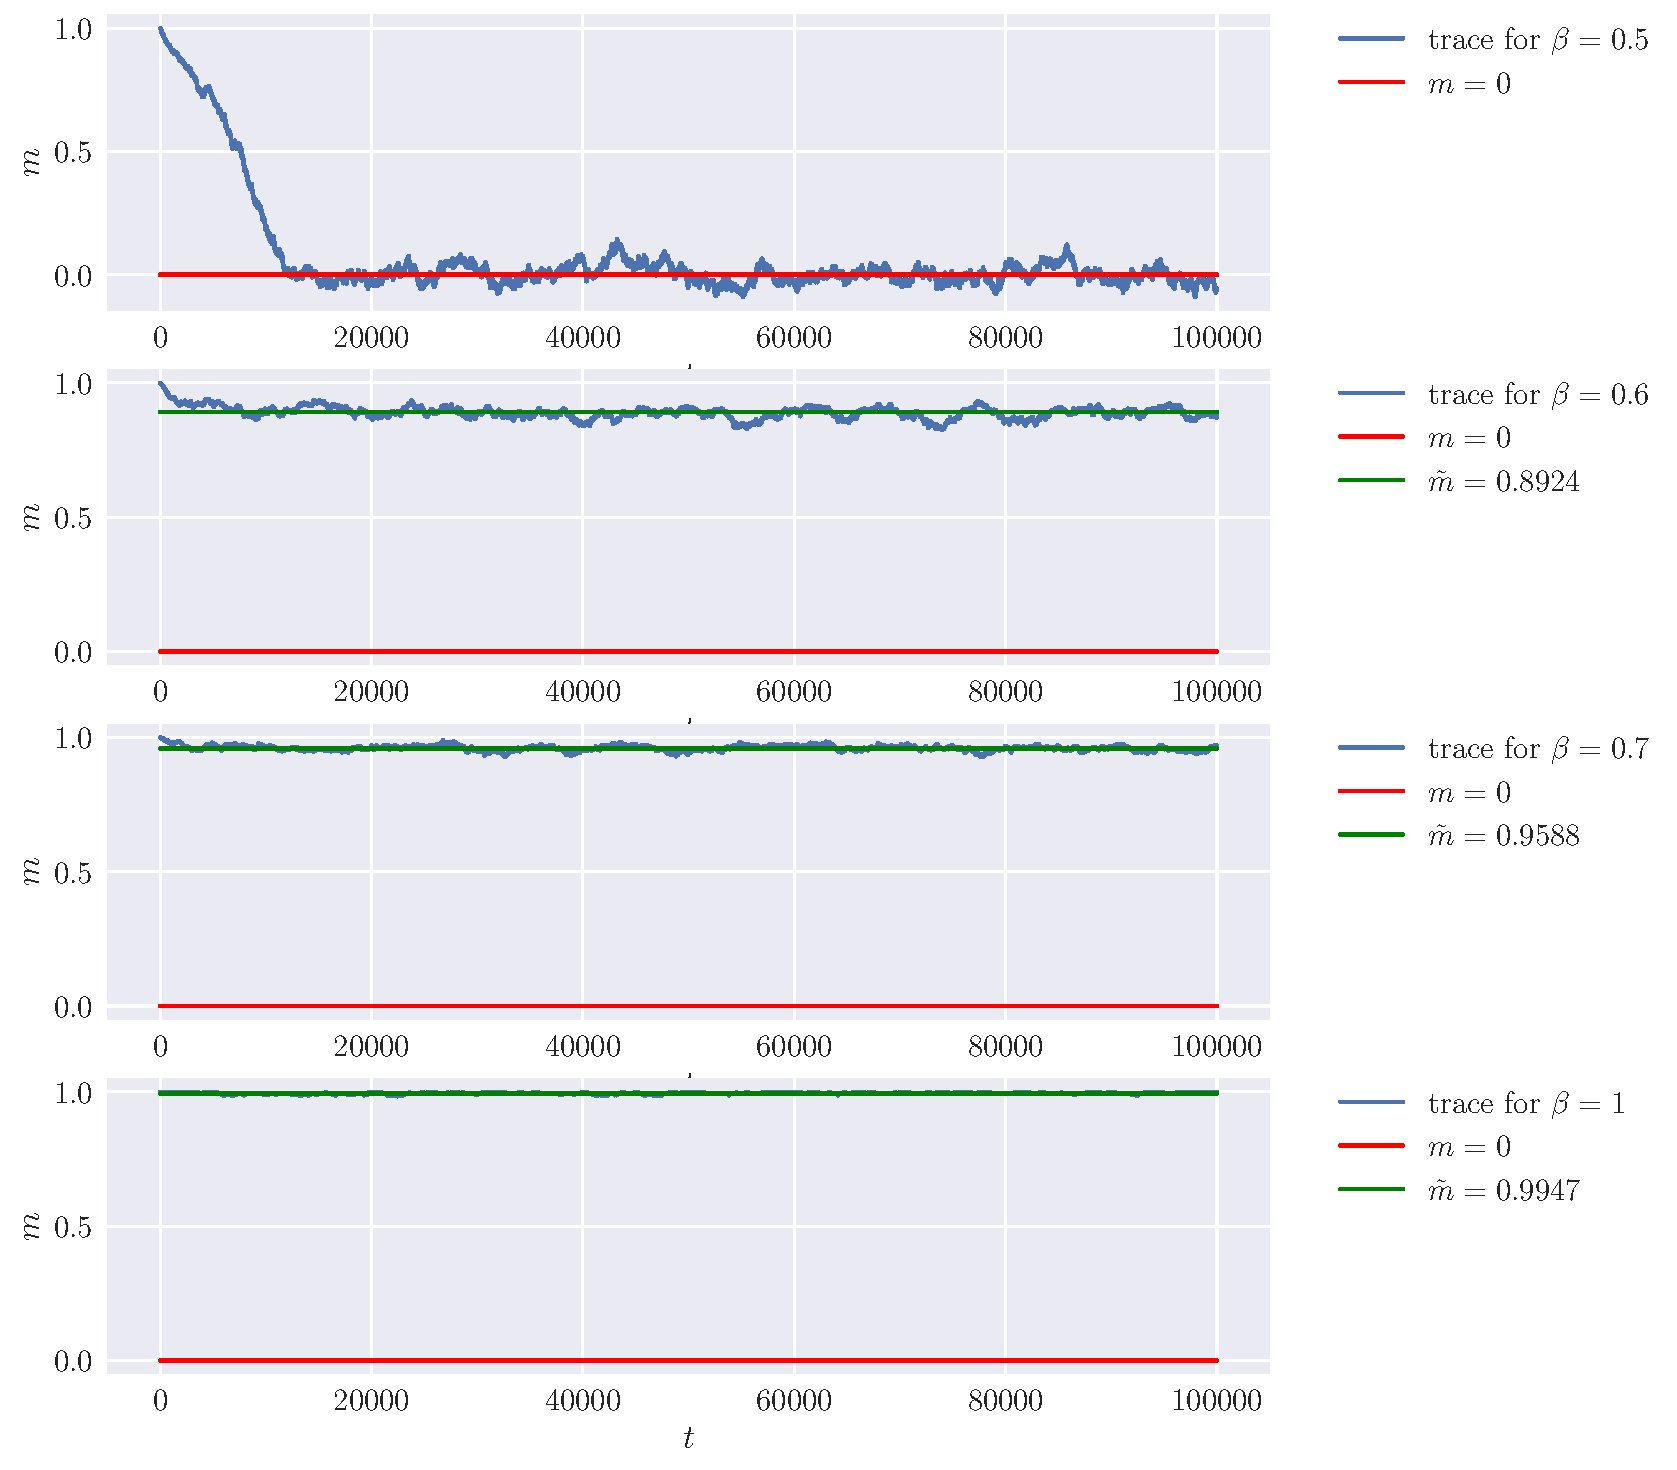
\includegraphics[width=500pt]{hw2/hw2_2(b)1.pdf}
%             \caption{Starting at all-plus configuration, i.e. $ m = 1 $, the trace plot under $ \beta = 0.5, 0.6, 0.7, 1 $}
%         \end{figure}
%         \begin{figure}
%             \centering
%             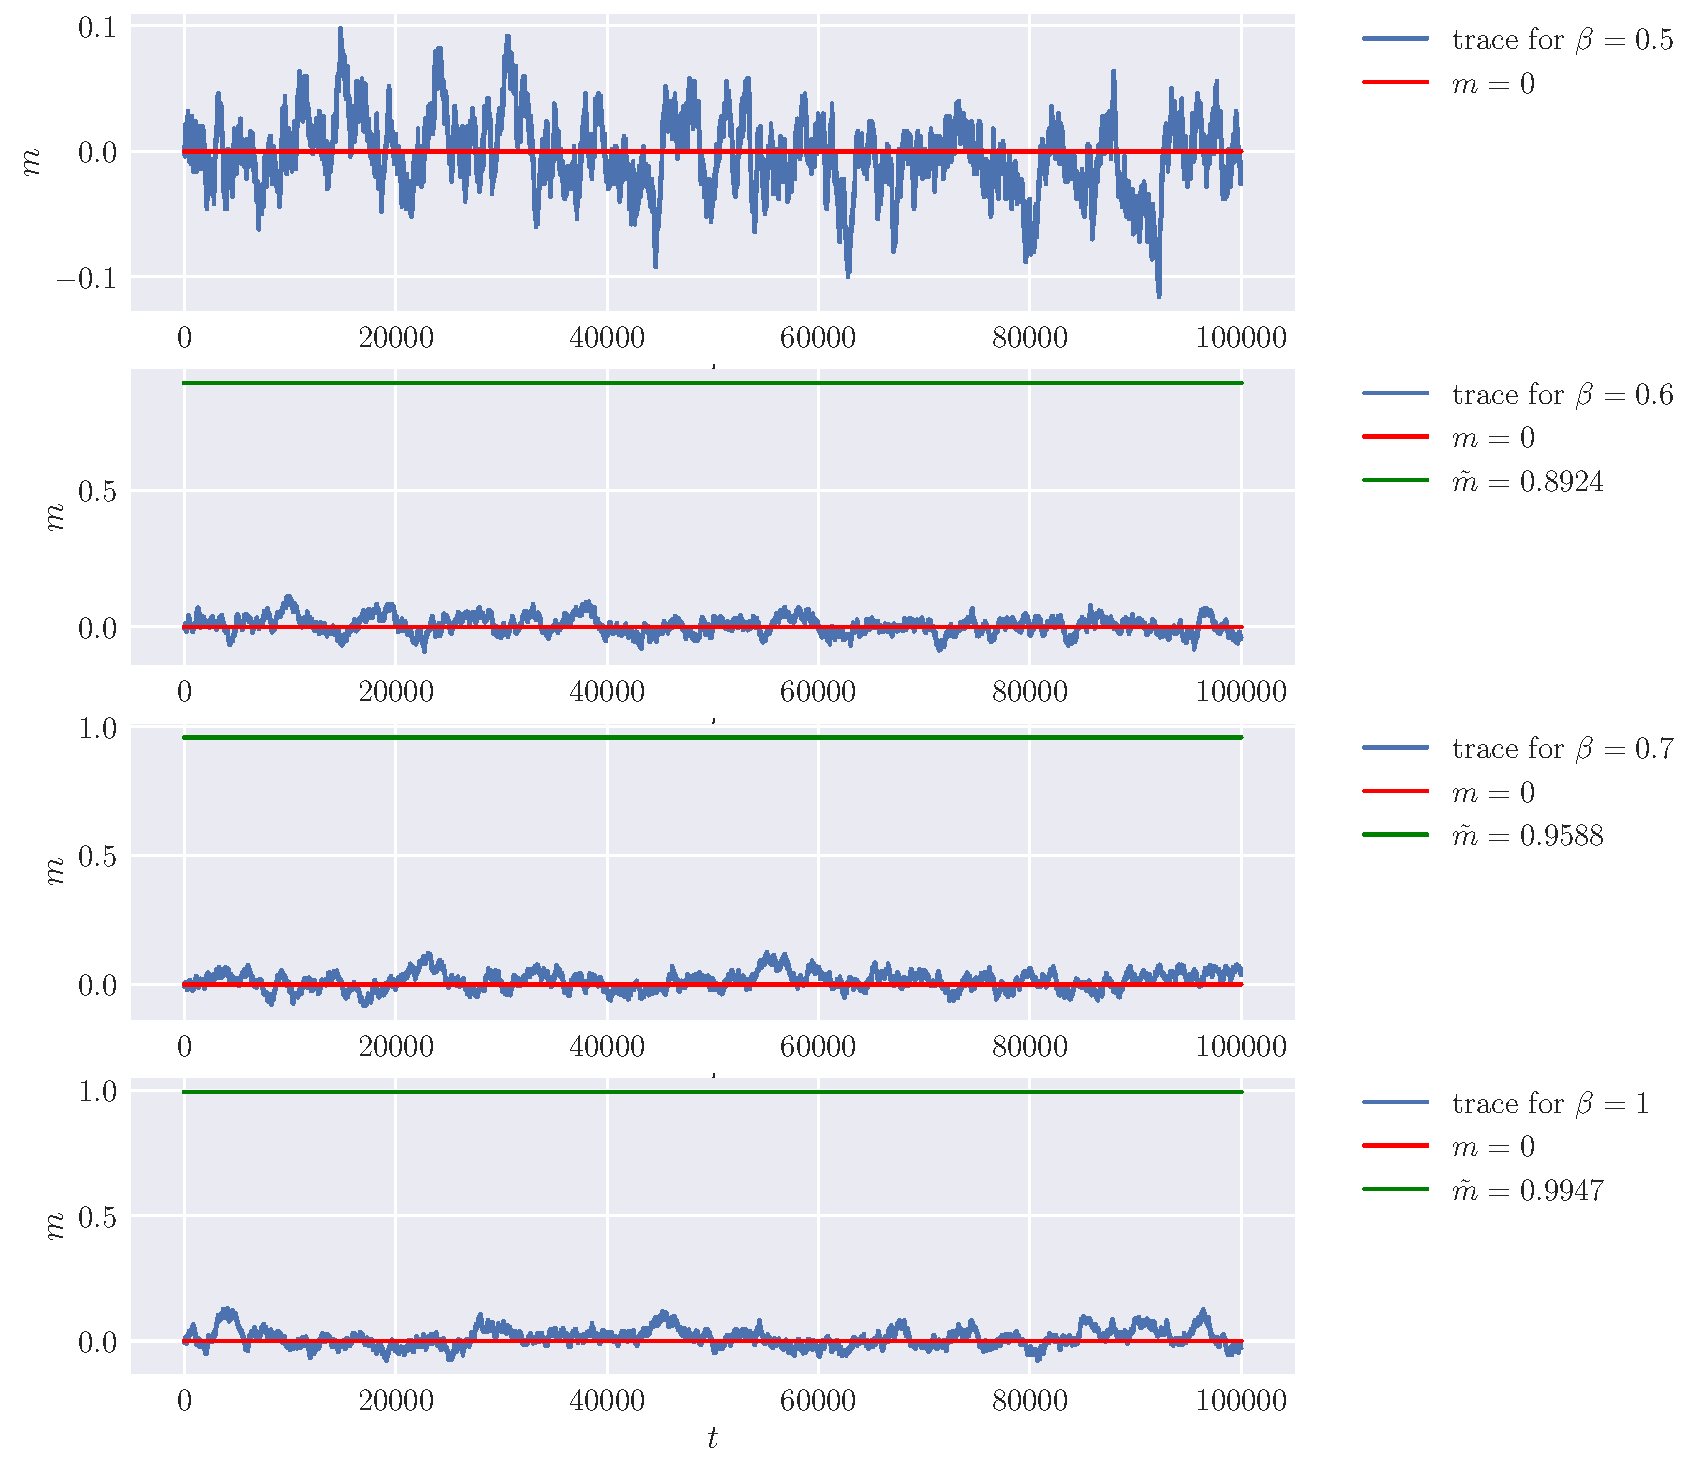
\includegraphics[width=500pt]{hw2/hw2_2(b)2.pdf}
%             \caption{Starting at half-minus-half-plus configuration, i.e. $ m = 0 $, the trace plot under $ \beta = 0.5, 0.6, 0.7, 1 $}
%         \end{figure}
% \item 
%         \def\mm{\mathsf{m}}
%         Define $ P(t, \mm) $ as the probability (over different realizations of the dynamics) that the value of the magnetization is $ M = N \mm $ at time $ t $, where $ -N \le M \le N $.
%         Its average value per spin is
%         \begin{equation*}
%             m(t) = \int_0^1  \dd \mm \, P(t, \mm) \, \mm
%         \end{equation*}
%         The master equation for $ P(t,\mm) $ reads
%         \begin{IEEEeqnarray*}{rCl}
%             P(t + \delta t, \mm)
%             &=& \frac{ 1 + \rdbrs{ \mm + \frac{2}{N} } }{2} p_- \rdbrs{ \mm + \frac{2}{N} } P \rdbrs{ t, \mm + \frac{2}{N} } \\
%             && + \frac{ 1 - \rdbrs{ \mm - \frac{2}{N} } }{2} p_+ \rdbrs{ \mm - \frac{2}{N} } P \rdbrs{ t, \mm - \frac{2}{N} }  \\
%             && + \sqbrs{ \frac{1+\mm}{2} p_+(\mm) + \frac{1-\mm}{2} p_-(\mm) } P(t, \mm) \\
%         \end{IEEEeqnarray*}
%         Therefore, plug in $ p_\pm $, the average magnetization at time $ t + \dd t $ is 
%         \begin{IEEEeqnarray*}{rCl}
%             m(t + \delta t)
%             &=& \int_0^1 \dd \mm \, P(t + \delta t, \mm) \, \mm \\
%             &=& \int_0^1 \dd \mm \sqbrs{ \frac{ 1 + \rdbrs{ \mm + \frac{2}{N} } }{2} p_- \rdbrs{ \mm + \frac{2}{N} } P \rdbrs{ t, \mm + \frac{2}{N} } } \mm \\
%             && + \int_0^1 \dd \mm \sqbrs{ \frac{ 1 - \rdbrs{ \mm - \frac{2}{N} } }{2} p_- \rdbrs{ \mm - \frac{2}{N} } P \rdbrs{ t, \mm - \frac{2}{N} } } \mm \\
%             && + \int_0^1 \dd \mm \sqbrs{ \frac{1+\mm}{2} p_+(\mm) + \frac{1-\mm}{2} p_-(\mm) } P(t, \mm) \, \mm \\
%             &=& \int_0^1 \dd \mm \sqbrs{ \frac{ 1 + \mm }{2} p_-(\mm) P(t, \mm) } \rdbrs{ \mm - \frac{2}{N} } \\
%             && + \int_0^1 \dd \mm \sqbrs{ \frac{ 1 - \mm }{2} p_-(\mm) P(t, \mm) } \rdbrs{ \mm + \frac{2}{N} } \\
%             && + \int_0^1 \dd \mm \sqbrs{ \frac{1+\mm}{2} p_+(\mm) + \frac{1-\mm}{2} p_-(\mm) } P(t, \mm) \, \mm \\
%             &=& \int_0^1 \dd \mm \clbrs{ \mm + \frac{2}{N} \sqbrs{ \frac{1-\mm}{2} p_+(\mm) - \frac{1+m}{2} p_-(\mm) } } P(t,\mm) + \mathrm{o} \rdbrs{ \frac{1}{N} } \\
%             &=& \int_0^1 \dd \mm \clbrs{ \mm - \frac{1}{N} \sqbrs{ \mm - \tanh(3 \beta \mm^2) } } P(t, \mm) + \mathrm{o} \rdbrs{ \frac{1}{N} }
%         \end{IEEEeqnarray*}
%         where the team $ \mathrm{o} \rdbrs{ \frac{1}{N} } $ is introduced by change of variable but keep the integrate range fixed.

%         Considering that fluctuations in $ m $ are $ \mathrm{O} \rdbrs{ 1/\sqrt{N} } $, by setting $ \delta t = 1/N $ and let $ N \to \infty $, we have
%         \begin{IEEEeqnarray*}{rCl}
%             \fracd{}{t} m(t)
%             &=& \frac{ m(t + \delta t) - m(t) }{ \delta t } 
%             = \int \dd \mm \sqbrs{ \tanh(3 \beta \mm^2) - \mm } P(t, \mm) 
%             = \tanh \rdbrs{ 3 \beta \sqbrs{ m(t) }^2 } - m(t)
%         \end{IEEEeqnarray*}
% \end{enumerate}
% \end{solution}

\subsection*{B. Bethe free entropy }

\begin{enumerate}[(a)]
\item 
        Show from the generic formula for Bethe free entropy per spin that we derived in the lecture
        \begin{equation*}
            f_{\mathrm{Bethe}}^{\mathrm{general}}
            = \frac{1}{N} \sum_{i=1}^N \log(Z^i) + \frac{1}{N} \sum_{a=1}^M \log(Z^a) - \frac{1}{N} \sum_{ia} \log(Z^{ia}) \tag{$\dagger$}
        \end{equation*}
        where
        \begin{IEEEeqnarray*}{rCl}
            Z^i &=& \sum_s g_i(s) \prod_{a \in \partial i} \psi_s^{a \to i} \\
            Z^a &=& \sum_{ \clbrs{ s_i }_{i \in \partial a} } f_a \rdbrs{ \clbrs{ s_i }_{i \in \partial a} } \prod_{i \in \partial a} \chi_{s_i}^{i \to a} \\
            Z^{ia} &=& \sum_s \psi_s^{a \to i} \chi_s^{i \to a}
        \end{IEEEeqnarray*}
        that the Bethe free entropy for graph coloring can be written as
        \begin{equation*}
            f_{\mathrm{Bethe}}^{\mathrm{coloring}}
            = \frac{1}{N} \sum_{i=1}^N \log \rdbrs{ Z^{(i)} } - \frac{1}{N} \sum_{(ij) \in E} \log \rdbrs{ Z^{(ij)} }
        \end{equation*}
        where
        \begin{IEEEeqnarray*}{rCl}
            Z^{(i)} &=& \sum_s \prod_{k \in \partial i} \sqbrs{ 1 - \rdbrs{ 1 - \ee^{-\beta} } \chi_s^{k \to i} } \\
            Z^{(ij)} &=& 1 - \rdbrs{ 1 - \ee^{-\beta} } \sum_s \chi_s^{i \to (ij)} \chi_s^{j \to (ij)} 
        \end{IEEEeqnarray*}
\item
        \textbf{A key connection between Belief Propagation and the Bethe free entropy}: \\
        Show that the BP equations we derived in the lecture 
        \begin{IEEEeqnarray*}{rCl}
            \chi_{s_j}^{j \to a}
            &=& \frac{1}{Z^{j \to a}} g_j(s_j) \prod_{b \in \partial j \setminus a} \psi_{s_j}^{b \to j} \\
            \psi_{s_i}^{a \to i}
            &=& \frac{1}{Z^{a \to i}} \sum_{\clbrs{ s_j }_{j \in \partial a \setminus i}} f_a \rdbrs{ \clbrs{ s_j }_{j \in \partial a} } \prod_{j \in \partial a \setminus i} \chi_{s_j}^{j \to a}
        \end{IEEEeqnarray*}
        are stationarity conditions of the Bethe free entropy $ (\dagger) $ under the constraint that both $ \sum_s \psi^{a\to i}_s = 1 $ and $ \sum_s \chi^{i\to a}_s = 1 $ for all $ (ia) \in E $.
\end{enumerate}
\begin{solution} $\,$ 
\begin{enumerate}[(a)]
\item 
        Given graph $ G(V,E) $, let's define its associated factor graph $ \mathsf{FG}(\tilde{V}, \tilde{F}, \tilde{E}) $, where
        \begin{itemize}
        \item   $ \tilde{V} = V $ is the set of variable nodes in factor graph, the value is the color of the corresponding node
        \item   $ \tilde{F} = E $ is the set of factor nodes in factor graph, the constraint function is $ f_{ij}(s_i, s_j) = \mathbb{I}(s_i \ne s_j) $.
                However, since the indicator constraint function is hard to deal with, usually we soften the constraint as $ f_{ij}(s_i, s_j) = \ee^{-\beta \, \mathbb{I}(s_i = s_j)} $ and let $ \beta \to \infty $.
        \item   $ \tilde{E} = \bigcup_{ (ij) \in E } \clbrs{ (i,ij), (j,ij) } $ is the set of edges in factor graph
        \end{itemize}
        The Boltzmann distribution of the factor graph is
        \begin{equation*}
            P \rdbrs{ \clbrs{ s_i }_{i=1}^N }
            = \frac{1}{Z} \prod_{ (ij) \in \tilde{F} } f_{ij}(s_i, s_j)
            = \frac{1}{Z} \prod_{ (ij) \in E } \ee^{-\beta \, \mathbb{I} \rdbrs{ s_i = s_j } }
        \end{equation*}
        Notice that in this factor graph, every factor node has exactly degree $ 2 $, this type of model is called \emph{pair-wise model}.
        According to BP rule we have
        \begin{IEEEeqnarray*}{rCl}
            \psi_{s_i}^{(ij) \to i} 
            &=& \frac{1}{\tilde{Z}^{(ij) \to i}} \sum_{s_j} f_{ij}(s_i, s_j) \chi_{s_j}^{j \to (ij)} 
            = \frac{1}{\tilde{Z}^{(ij) \to i}} \sqbrs{ f_{ij}(s_i, s_i) \chi_{s_i}^{j \to (ij)} + \sum_{s_j \ne s_j} f_{ij}(s_i, s_j) \chi_{s_j}^{j \to (ij)} } \\
            &=& \frac{ \ee^{-\beta} \chi_{s_i}^{j \to (ij)} + \sum_{s_j \ne s_i} \chi_{s_j}^{j \to (ij)} }{ \tilde{Z}^{(ij) \to i} }
            = \frac{ 1 - (1-\ee^{-\beta}) \chi_{s_i}^{j \to (ij)} \ztag{$*$} }{\tilde{Z}^{(ij) \to i}}
        \end{IEEEeqnarray*}
        where $ \tilde{Z}^{(ij) \to i} $ is the normalization constant of $ \psi_{s_i}^{(ij) \to i} $.

        Hence, it is sufficient to only use one set of BP messages, here we choose $ \chi $'s.

        Besides, to distinguish the neighborhood of node $ i $ in $ G(V,E) $ and the neighborhood of variable node $ i $ in $ \mathsf{FG}(\tilde{V}, \tilde{F}, \tilde{E}) $, I will use $ \partial^* i $ to denote the neighborhood in $ G(V,E) $, i.e.
        \begin{equation*}
            \partial^* i = \clbrsv{ j }{ (ij) \in E }, \qquad
            \partial i = \clbrsv{ (ij) }{ (i, ij) \in \tilde{E} }
        \end{equation*}

        Therefore, start from $ (\dagger) $ we have
        \begin{IEEEeqnarray*}{rCl}
            f_{\mathrm{Bethe}}^{\mathrm{coloring}}
            &=& \frac{1}{N} \sum_{i \in \tilde{V}} \log(\tilde{Z}^{(i)}) + \frac{1}{N} \sum_{(ij) \in \tilde{F}} \log(\tilde{Z}^{(ij)}) - \frac{1}{N} \sum_{ (i,ij) \in \tilde{E} } \log(\tilde{Z}^{(i,ij)}) \\
            &=& \frac{1}{N} \sum_{i=1}^N \log(\tilde{Z}^{(i)}) + \frac{1}{N} \sum_{(ij) \in E} \log(\tilde{Z}^{(ij)}) - \frac{1}{N} \sum_{ (ij) \in E } \sqbrs{ \log(\tilde{Z}^{(i,ij)}) + \log(\tilde{Z}^{(j,ij)}) } \ztag{$\ddagger$}
        \end{IEEEeqnarray*}
        where
        \begin{IEEEeqnarray*}{rCl}
            \tilde{Z}^{(i)} 
            &=& \sum_s \prod_{(ik) \in \partial i} \psi_s^{(ik) \to i}
            \texteq{\text{by } (*)} \sum_s \prod_{k \in \partial^* i} \frac{ 1 - \rdbrs{ 1 - \ee^{-\beta} } \chi_s^{(ik) \to i} }{ \tilde{Z}^{(ik) \to i} }
            = \frac{ Z^{(i)} }{ \prod_{k \in \partial^* i} \tilde{Z}^{(ik) \to i} } \\
            \tilde{Z}^{(ij)} 
            &=& \sum_{s_i, s_j} f_{ij} \rdbrs{s_i, s_j} \chi_{s_i}^{i \to (ij)} \chi_{s_j}^{j \to (ij)}
            = \ee^{-\beta} \sum_s \chi_s^{i \to (ij)} \chi_s^{j \to (ij)} + \sum_{s_i \ne s_j} \chi_{s_i}^{i \to (ij)} \chi_{s_j}^{j \to (ij)} \\
            &=& \rdbrs{ \ee^{-\beta} - 1 } \sum_s \chi_s^{i \to (ij)} \chi_s^{j \to (ij)} + \sum_{s_i} \chi_{s_i}^{i \to (ij)} \cdot \sum_{s_j} \chi_{s_j}^{j \to (ij)} \\
            &=& 1 - \rdbrs{ 1 - \ee^{-\beta} } \sum_s \chi_s^{i \to (ij)} \chi_s^{j \to (ij)} 
            = Z^{(ij)} \\
            \tilde{Z}^{(i,ij)} 
            &=& \sum_s \psi_s^{(ij) \to i} \chi_s^{i \to (ij)}
            = \frac{1}{\tilde{Z}^{(ij) \to i}} \sum_s \sqbrs{ 1 - \rdbrs{ 1 - \ee^{-\beta} } \chi_s^{(ij) \to i} } \chi_s^{i \to (ij)} \\
            &=& \frac{1}{\tilde{Z}^{(ij) \to i}} \sqbrs{ 1 - \rdbrs{ 1 - \ee^{-\beta} } \sum_s \chi_s^{i \to (ij)} \chi_s^{j \to (ij)} }
            = \frac{ Z^{(ij)} }{ \tilde{Z}^{(ij) \to i} }
        \end{IEEEeqnarray*}
        Finally, substituting equations above back to $ (\ddagger) $ yields
        \begin{IEEEeqnarray*}{rCl}
            f_{\mathrm{Bethe}}^{\mathrm{coloring}}
            &=& \frac{1}{N} \sum_{i=1}^N \sqbrs{ \log(Z^{(i)}) - \sum_{k \in \partial^* i} \log \rdbrs{ \tilde{Z}^{(ik) \to i} } } + \frac{1}{N} \sum_{(ij) \in E} \log(Z^{(ij)}) \\
            && - \frac{1}{N} \sum_{(ij) \in E} \sqbrs{ \log(Z^{(ij)}) - \log(\tilde{Z}^{(ij) \to i}) + \log(Z^{(ij)}) - \log(\tilde{Z}^{(ij) \to j}) } \\
            &=& \frac{1}{N} \log \rdbrs{ Z^{(i)} } - \frac{1}{N} \sum_{(ij) \in E} \log \rdbrs{ Z^{(ij)} }
        \end{IEEEeqnarray*}
        since the sum $ \sum_{i=1}^N \sum_{k \in \partial^* i} $ counts each edge twice ($ (ij) $ and $ (ji) $).

        The proof is finished by simplify the notation $ \chi_s^{i \to (ij)} $ to $ \chi_s^{i \to j} $.
\item   
        To compute the stationarity conditions of Bethe free entropy, we start from taking partial derivative w.r.t. every BP message components $ \chi_{s_i}^{i \to a} $ and $ \psi_{s_i}^{a \to i} $ for all $ i \in [N] $, $ a \in [M] $ and $ s_i \in \mathcal{X} $, where $ \mathcal{X} $ is the alphabet of spin.
        \begin{IEEEeqnarray*}{rCl}
            N \fracp{}{\chi_{s_i}^{i \to a}} f_{\mathrm{Bethe}}^{\mathrm{general}}
            &=& \fracp{}{\chi_{s_i}^{i \to a}} \log \rdbrs{ Z^a } - \fracp{}{\chi_{s_i}^{i \to a}} \log \rdbrs{ Z^{ia} } \\
            &=& \frac{ \sum_{ \clbrs{ s_k }_{k \in \partial a \setminus i} } f_a \rdbrs{ s_i, \clbrs{ s_k }_{k \in \partial a \setminus i} } \prod_{k \in \partial a \setminus i} \chi_{s_k}^{k \to a} }{ \sum_{ \clbrs{ s_k }_{k \in \partial a} } f_a \rdbrs{ \clbrs{ s_k }_{k \in \partial a} } \prod_{k \in \partial a} \chi_{s_k}^{k \to a} }
            - \frac{ \psi_{s_i}^{a \to i} }{ \sum_s \psi_s^{a \to i} \chi_s^{i \to a} } \\
            N \fracp{}{\psi_{s_i}^{a \to i}} f_{\mathrm{Bethe}}^{\mathrm{general}}
            &=& \fracp{}{\psi_{s_i}^{a \to i}} \log \rdbrs{ Z^i } - \fracp{}{\psi_{s_i}^{a \to i}} \log \rdbrs{ Z^{ia} } \\
            &=& \frac{ g_i(s_i) \prod_{c \in \partial i \setminus a} \psi_{s_i}^{c \to i} }{ \sum_s g_i(s) \prod_{a \in \partial i} \psi_s^{a \to i} }
            - \frac{ \chi_{s_i}^{i \to a} }{ \sum_s \psi_s^{a \to i} \chi_s^{i \to a} }
        \end{IEEEeqnarray*}
        Setting these partial derivatives to zero and using the normalization constraints gives
        \begin{IEEEeqnarray*}{rCl}
            \psi_{s_i}^{a \to i}
            &=& \underbrace{ \frac{ \sum_s \psi_s^{a \to i} \chi_s^{i \to a} }{ \sum_{ \clbrs{ s_k }_{k \in \partial a} } f_a \rdbrs{ \clbrs{ s_k }_{k \in \partial a} } \prod_{k \in \partial a} \chi_{s_k}^{k \to a} } }_{\text{independent of } s_i} \sum_{ \clbrs{ s_k }_{k \in \partial a \setminus i} } f_a \rdbrs{ \clbrs{ s_k }_{k \in \partial a} } \prod_{k \in \partial a \setminus i} \chi_{s_k}^{k \to a} \\
            \psi_{s_i}^{a \to i}
            &=& \frac{ \psi_{s_i}^{a \to i} }{ \sum_s \psi_s^{a \to i} }
            = \frac{ \sum_{ \clbrs{ s_k }_{k \in \partial a \setminus i} } f_a \rdbrs{ \clbrs{ s_k }_{k \in \partial a} } \prod_{k \in \partial a \setminus i} \chi_{s_k}^{k \to a} }{ \underbrace{ \sum_{ \clbrs{ s_k }_{k \in \partial a} } f_a \rdbrs{ \clbrs{ s_k }_{k \in \partial a} } \prod_{k \in \partial a \setminus i} \chi_{s_k}^{k \to a} }_{=Z^{a \to i}} } \\
            \chi_{s_i}^{i \to a}
            &=& \underbrace{ \frac{ \sum_s \psi_s^{a \to i} \chi_s^{i \to a} }{ \sum_{s} g_i(s) \prod_{c \in \partial i} \psi_{s}^{c \to i} } }_{\text{independent of } s_i} g_i(s_i) \prod_{c \in \partial i \setminus a} \psi_{s_i}^{c \to i} \\
            \chi_{s_i}^{i \to a}
            &=& \frac{ \chi_{s_i}^{i \to a} }{ \sum_s \chi_s^{i \to a} } 
            = \frac{ g_i(s_i) \prod_{c \in \partial i \setminus a} \psi_{s_i}^{c \to i} }{ \underbrace{ \sum_{s} g_i(s) \prod_{c \in \partial i \setminus a} \psi_{s}^{c \to i} }_{=Z^{i \to a}} }
        \end{IEEEeqnarray*}
        Finally we have the stationarity conditions for Bethe free entropy, for all $ i \in [N], a \in [M] $ and $ s_i \in \mathcal{X} $
        \begin{IEEEeqnarray*}{rCl}
            \psi_{s_i}^{a \to i}
            &=& \frac{1}{Z^{a \to i}} \sum_{ \clbrs{ s_k }_{k \in \partial a \setminus i} } f_a \rdbrs{ \clbrs{ s_k }_{k \in \partial a} } \prod_{k \in \partial a \setminus i} \chi_{s_k}^{k \to a} \\
            \chi_{s_i}^{i \to a}
            &=& \frac{1}{Z^{i \to a}} g_i(s_i) \prod_{c \in \partial i \setminus a} \psi_{s_i}^{c \to i}
        \end{IEEEeqnarray*}
        which is exactly identical to BP equations.
\end{enumerate}
\end{solution}


\subsection*{C. Belief propagation for the k-factor problem on random graphs}

Consider now the $ k $-factor problem on random Erd\H{o}s-R\'{e}nyi graphs of average degree $ c = \mathrm{O}(1) $. 
Use the graphical model representation from the previous homeworks. 

\begin{enumerate}[(a)]
\item 
        Write belief propagation equations able to estimate the marginals of the probability distribution
        \begin{equation*}
            P \rdbrs{ \clbrs{ S_{(ij)} }_{(ij) \in E} }
            = \frac{1}{Z(\beta)} \prod_{(ij) \in E} \ee^{\beta S_{(ij)}} \prod_{i=1}^N \mathbb{I} \rdbrs{ \sum_{j \in \partial i} S_{(ij)} \le k }
        \end{equation*}
        Be careful that in the $ k $-factor model the nodes of the graph play the role of factor nodes in the graphical model and edges in the graph carry the variables nodes in the graphical model. 
\item 
        Write the corresponding Bethe free entropy in order to estimate $ \log (Z(\beta)) $. 
        Use results of the previous homework to suggest how to estimate the number of $ k $-factors of a given size $ s(e) $ on a given randomly generated large graph $ G $. 
\item  
        Consider now $ d $-regular random graphs and express the plot $ s(e) $ for $ k = 1,2,3 $, for several values of $ d $.
        Comment on what you obtained, does it correspond to your expectation from the previous homework?
        If now, explain the differences.
\item 
        \textbf{BONUS} Implement the BP equations and compute the $ s(e) $ for the $ k $-factor model on a given random Erd\H{o}s-R\'{e}nyi graph.
        Plot $ s(e) $ for several values of the average degree $ c $ and $ k = 1 $ and $ 2 $.
\end{enumerate}
\begin{solution} $\,$ 
\begin{enumerate}[(a)]
\item 
        Given graph $ G(V,E) $, let's define its associated factor graph $ \mathsf{FG}(\tilde{V}, \tilde{F}, \tilde{E}) $, where
        \begin{itemize}
        \item   $ \tilde{V} = E $ is the set of variable nodes in factor graph.
                Given any $ \mathsf{M} \subseteq E $, the values $ S_{(ij)} \in \clbrs{0, 1} $ represent whether edge $ (ij) \in \mathsf{M} $ or not.
        \item   $ \tilde{F} = V $ is the set of factor nodes in factor graph.
                The constraint function is
                \begin{equation*}
                    f_i \rdbrs{ \clbrs{ S_{(ij)} }_{j \in \partial^* i} } 
                    = \mathbb{I} \rdbrs{ \sum_{j \in \partial^* i} S_{(ij)} \le k }
                \end{equation*}
        \item   $ \tilde{E} = \bigcup_{ (ij) \in E } \clbrs{ (ij,i), (ij,j) } $ is the set of edges in factor graph.
        \end{itemize}
        Therefore, the BP equations
        \begin{IEEEeqnarray*}{rCl}
            \psi_{S_{(ij)}}^{i \to (ij)}
            &=& \frac{1}{Z^{i \to (ij)}} \sum_{ \clbrs{ S_{(il)} }_{(il) \in \partial i \setminus (ij)} } f_i \rdbrs{ \clbrs{ S_{(il)} }_{(il) \in \partial i} } \prod_{(il) \in \partial i \setminus (ij)} \chi_{S_{(il)}}^{(il) \to i} \\
            &=& \frac{1}{Z^{i \to (ij)}} \sum_{ \clbrs{ S_{(il)} }_{l \in \partial^* i \setminus j} } \mathbb{I} \rdbrs{ \sum_{l \in \partial^* i} S_{(il)} \le k } \prod_{l \in \partial^* i \setminus j} \chi_{S_{(il)}}^{(il) \to i} \\
            \chi_{S_{(ij)}}^{(ij) \to i}
            &=& \frac{1}{Z^{(ij) \to i}} g_{ij}(S_{(ij)}) \prod_{c \in \partial (ij) \setminus i} \psi_{S_{(ij)}}^{c \to (ij)} 
            = \frac{1}{Z^{(ij) \to i}} \ee^{\beta S_{(ij)}} \psi_{S_{(ij)}}^{j \to (ij)}
        \end{IEEEeqnarray*}
        where $ Z^{i \to (ij)} $ and $ Z^{(ij) \to i} $ are normalization constants to ensure
        \begin{equation*}
            \sum_s \psi_s^{i \to (ij)} = 1, \qquad
            \sum_s \chi_s^{(ij) \to i} = 1
        \end{equation*}
\item   
        Before we write the Bethe free entropy, let's first write down each component separately
        \begin{IEEEeqnarray*}{rCCl}
            \text{For variable nodes} \quad
            &Z^{(ij)} 
            &=& \sum_s g_{ij}(s) \prod_{c \in \partial (ij)} \psi_s^{c \to {(ij)}} 
            = \sum_s \ee^{\beta s} \psi_s^{i \to (ij)} \psi_s^{j \to (ij)} \\
            \text{For factor nodes} \quad
            &Z^i 
            &=& \sum_{ \clbrs{ s_{(ij)} }_{j \in \partial^* i} } f_i \rdbrs{ \clbrs{ s_{(ij)} }_{j \in \partial^* i} } \prod_{j \in \partial^* i} \chi_{s_{(ij)}}^{(ij) \to i} \\
            &&=& \sum_{ \clbrs{ s_{(ij)} }_{j \in \partial^* i} } \mathbb{I} \rdbrs{ \sum_{j \in \partial^* i} S_{(ij)} \le k } \prod_{j \in \partial^* i} \chi_{s_{(ij)}}^{(ij) \to i} \\
            \text{For edges} \quad
            &Z^{(ij), i} &=& \sum_s \psi_s^{i \to (ij)} \chi_s^{(ij) \to i}
        \end{IEEEeqnarray*}
        Hence, the Bethe free entropy for $ k $-factor problem at inverse temperature $ \beta $ is
        \begin{IEEEeqnarray*}{rCl}
            f_{\mathrm{Bethe}}^{k\text{-factor}}(\beta)
            = \frac{1}{N} \clbrs{ \sum_{(ij) \in E} \log \rdbrs{ Z^{(ij)} } + \sum_{i=1}^N \log \rdbrs{ Z^i } - \sum_{(ij) \in E} \sqbrs{ \log \rdbrs{ Z^{(ij),i} } + \log \rdbrs{ Z^{(ij),j} } } }
        \end{IEEEeqnarray*}
        According to HW1, what we want to compute is the free entropy density
        \begin{equation*}
            f(\beta) = \limit{N \to \infty} \frac{\log(Z(\beta))}{N}
        \end{equation*}
        Since as $ N \to \infty $, the Erd\H{o}s-R\'enyi graphs are locally tree-like, the Bethe free entropy per spin is asymptotically close to the true free entropy density, i.e.
        \begin{equation*}
            f(\beta) \approx f_{\mathrm{Bethe}}^{k\text{-factor}}(\beta)
        \end{equation*}
        Therefore, to compute $ s(e) $, we need to do the following steps
        \begin{enumerate}[1)]
        \item   Run BP long enough to reach equilibrium to get BP messages $ \chi $'s and $ \psi $'s.
        \item   Use the BP messages to compute Bethe free entropy per spin $ f_{\mathrm{Bethe}}^{k\text{-factor}}(\beta) $ as an approximation of the free entropy density $ f(\beta) $
        \item   Use conclusion of HW1, compute $ s(e) = \inf_{\beta \in \mathbb{R}} \sqbrs{ f(\beta) - \beta e } $
        \end{enumerate}
\item   
        For a $ d $-regular graph, in its associated factor graph, every variable node has degree $ 2 $, every factor node has degree $ d $.
        The local structure of each variable node and factor node are same thus we do need to distinguish them.
        Hence, denote $ \chi_s^{(ij) \to i} \equiv \chi_s $ and $ \psi_s^{i \to (ij)} \equiv \psi_s $ for all $ (ij) \in E $ and $ s \in \clbrs{ \pm1 } $.
        The BP equations becomes
        \begin{IEEEeqnarray*}{rCl}
            \psi_s 
            &\propto& \sum_{ \clbrs{ s_l }_{l=1}^{d-1} } \mathbb{I} \rdbrs{ s + \sum_{l=1}^{d-1} s_l \le k } \prod_{l=1}^{d-1} \chi_{s_l} \\
            &=& \sum_{\kappa=0}^{k-s}  \sum_{ \clbrs{ s_l }_{l=1}^{d-1} } \mathbb{I} \rdbrs{ \sum_{l=1}^{d-1} s_l = \kappa } \prod_{l=1}^{d-1} \chi_1^{s_l} \chi_0^{1-s_l} 
            = \sum_{\kappa=0}^{k-s} \binom{d-1}{\kappa} \chi_1^\kappa \chi_0^{d-1-\kappa} \\
            \psi_s 
            &=& \frac{ \sum_{\kappa=0}^{k-s} \binom{d-1}{\kappa} \chi_1^\kappa \chi_0^{d-1-\kappa} }{ \binom{d-1}{k} \chi_1^k \chi_0^{d-1-k} +  2\sum_{\kappa=0}^{k-1} \binom{d-1}{\kappa} \chi_1^\kappa \chi_0^{d-1-\kappa} } \\
            \chi_s
            &=& \frac{ \ee^{\beta s} \psi_s }{ \psi_0 + \ee^\beta \psi_1 }
            = \frac{ \ee^{\beta s} \psi_s }{ 1 + (\ee^\beta - 1) \psi_1 }
        \end{IEEEeqnarray*}
        Or, we can use a more compact parameterization: likelihood-ratio (LR), define
        \begin{equation*}
            h = \frac{\chi_1}{\chi_0}, \qquad \hat{h} = \frac{\psi_1}{\psi_0}
        \end{equation*}
        The BP equations become
        \begin{IEEEeqnarray*}{rCl}
            \hat{h} = \frac{ \sum_{\kappa=0}^{k-1} \binom{d-1}{\kappa} h^\kappa }{ \sum_{\kappa=0}^k \binom{d-1}{\kappa} h^\kappa }, \quad
            h = \ee^\beta \hat{h}
            \quad \Rightarrow \quad
            h = \ee^\beta \sqbrs{ 1 - \frac{ \binom{d-1}{k} h^k }{ \sum_{\kappa=0}^k \binom{d-1}{\kappa} h^\kappa } }
        \end{IEEEeqnarray*}

        Therefore, once we found the fixed point of $ h $ under certain $ \beta $, we can rewrite the Bethe free entropy of $ k $-factor problem on a random $ d $-regular graph at inverse temperature $ \beta $ can be computed as
        \begin{IEEEeqnarray*}{rCl}
            f_{\mathrm{Bethe}}^{k\text{-factor}}(\beta; d)
            &=& \frac{d}{2} \log \rdbrs{ \psi_0^2 + \ee^\beta \psi_1^2 } + \log \rdbrs{ \sum_{\kappa=0}^k \binom{d}{\kappa} \chi_1^\kappa \chi_0^{d-\kappa} } - d \log \rdbrs{ \psi_0 \chi_0 + \psi_1 \chi_1 } \\
            &=& \frac{d}{2} \beta - \frac{d}{2} \log \rdbrs{ \ee^\beta + h^2 } + \log \rdbrs{ \sum_{\kappa=0}^d \binom{d}{\kappa} h^\kappa }
        \end{IEEEeqnarray*}
        Then, to obtain the curve $ s(e) $, we can just use the procedure in part (b).

        The curve $ s(e) $ under $ k \in \clbrs{ 1,2,3 } $ and $ d \in \clbrs{ 3,4,5 } $ are given below
        \begin{figure}[H]
            \centering
            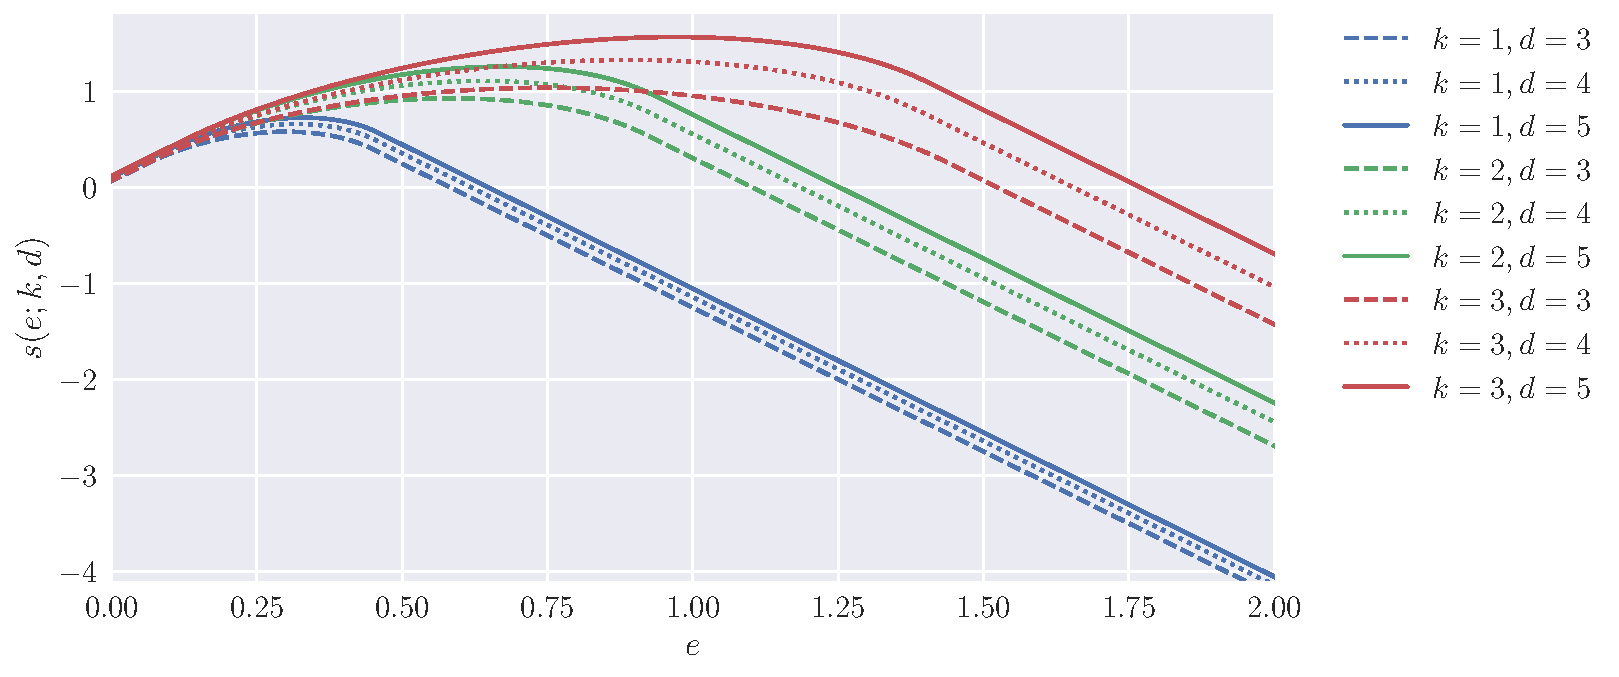
\includegraphics[width=450pt]{hw2/hw2_3(c).pdf}
        \end{figure}
        \begin{itemize}
        \item   Fix $ k $, the larger $ d $ is, the higher $ s(e; k, d) $ is.
        \item   Fix $ d $, the larger $ k $ is, the higher $ s(e; k, d) $ is. 
                When $ k \ge d $, every subset of edges is a valid $ k $-factor, and $ s(e; k, d) = H_\ee \rdbrs{ \frac{2e}{d} } $, where $ H_\ee(\cdot) $ is the binary entropy function under natural base.
        \item   As long as $ k < d $, there exists a $ e_{\mathrm{lin}} $ such that $ s(e; k, d) $ becomes linear when $ e > e_{\mathrm{lin}} $.
        \item   As long as $ k < d $, there exists a $ e_{\mathrm{sup}} $ such that $ s(e; k, d) < 0 $ for all $ e > e_{\mathrm{sup}} $, which means when $ N \to \infty $ there is no $ k $-factor with size $ e $ w.h.p. if $ e > e_{\mathrm{sup}} $.
        \end{itemize}
\item 
        Again, we use the same LR parameterization as part (c), the BP equation and Bethe free entropy can be written as
        \begin{IEEEeqnarray*}{rCl}
            h^{(ij) \to i} 
            &=& \ee^\beta \frac{ \sum_{\kappa=0}^{k-1} \sum_{ \substack{I \subseteq \partial^* i \setminus j \\ \abs{I} = \kappa } } \prod_{\ell \in I} h^{(i\ell) \to i} }{ \sum_{\kappa=0}^k \sum_{ \substack{I \subseteq \partial^* i \setminus j \\ \abs{I} = \kappa } } \prod_{\ell \in I} h^{(i\ell) \to i} } 
            = \ee^\beta \sqbrs{ 1 - \frac{ \sum_{ \substack{I \subseteq \partial^* i \setminus j \\ \abs{I} = k } } \prod_{\ell \in I} h^{(i\ell) \to i} }{ \sum_{ \substack{I \subseteq \partial^* i \setminus j \\ \abs{I} \le k } } \prod_{\ell \in I} h^{(i\ell) \to i} } } \\
            N f_{\mathrm{Bethe}}^{k\text{-factor}}(\beta; k, G)
            &=& \sum_{(ij) \in E} \log \clbrs{ \frac{ \ee^{2 \beta} + \ee^{\beta} h^{(ij) \to i} h^{(ij) \to j} }{ \rdbrs{ \ee^{\beta} + h^{(ij) \to i} } \rdbrs{ \ee^{\beta} + h^{(ij) \to j} } } } \\
            && + \sum_{i=1}^N \log \clbrs{ \sum_{\substack{ I \subseteq \partial^* i \\ \abs{I} \le k }} \prod_{j \in I} \frac{h^{(ij) \to i}}{1 + h^{(ij) \to i}} \prod_{j \in \partial^* i \setminus I} \frac{1}{1 + h^{(ij) \to i}} } \\
            && -\sum_{(ij) \in E} \sqbrs{ \log \clbrs{ \frac{ \ee^\beta + h^{(ij) \to i} h^{(ij) \to j} }{ \rdbrs{ 1 + h^{(ij) \to i} } \rdbrs{ \ee^\beta + h^{(ij) \to j} } } } + \log \clbrs{ \frac{ \ee^\beta + h^{(ij) \to j} h^{(ij) \to i} }{ \rdbrs{ 1 + h^{(ij) \to j} } \rdbrs{ \ee^\beta + h^{(ij) \to i} } } } } \\
            &=& \beta \abs{E} - \sum_{(ij) \in E} \log \rdbrs{ \ee^\beta + h^{(ij) \to i} h^{(ij) \to j} } 
            + \sum_{i=1}^N \log \rdbrs{ \sum_{ \substack{ I \subseteq \partial^* i \\ \abs{I} \le k } } \prod_{j \in I} h^{(ij) \to i} }
        \end{IEEEeqnarray*}
        The figure below gives the $ s(e) $ for three Erd\H{o}s-R\'enyi drawn from ensemble $ \mathbb{G}_{\mathrm{ER}}(N, c) $ with $ N = 1000 $ and $ c \in \clbrs{ 3,4,5 } $.
        For each sampled random graph, I ran BP for the $ k $-factor problem for $ k \in \clbrs{ 1,2,3 } $ and $ \beta \in [-3, 3] $ to compute $ f_{\mathrm{Bethe}}^{k\text{-factor}}(\beta; k, G) $.
        Finally, I apply Legendre transformation to get the $ s(e; k, c) $ curve for a $ (k, c) $ pair.
        \begin{figure}[H]
            \centering
            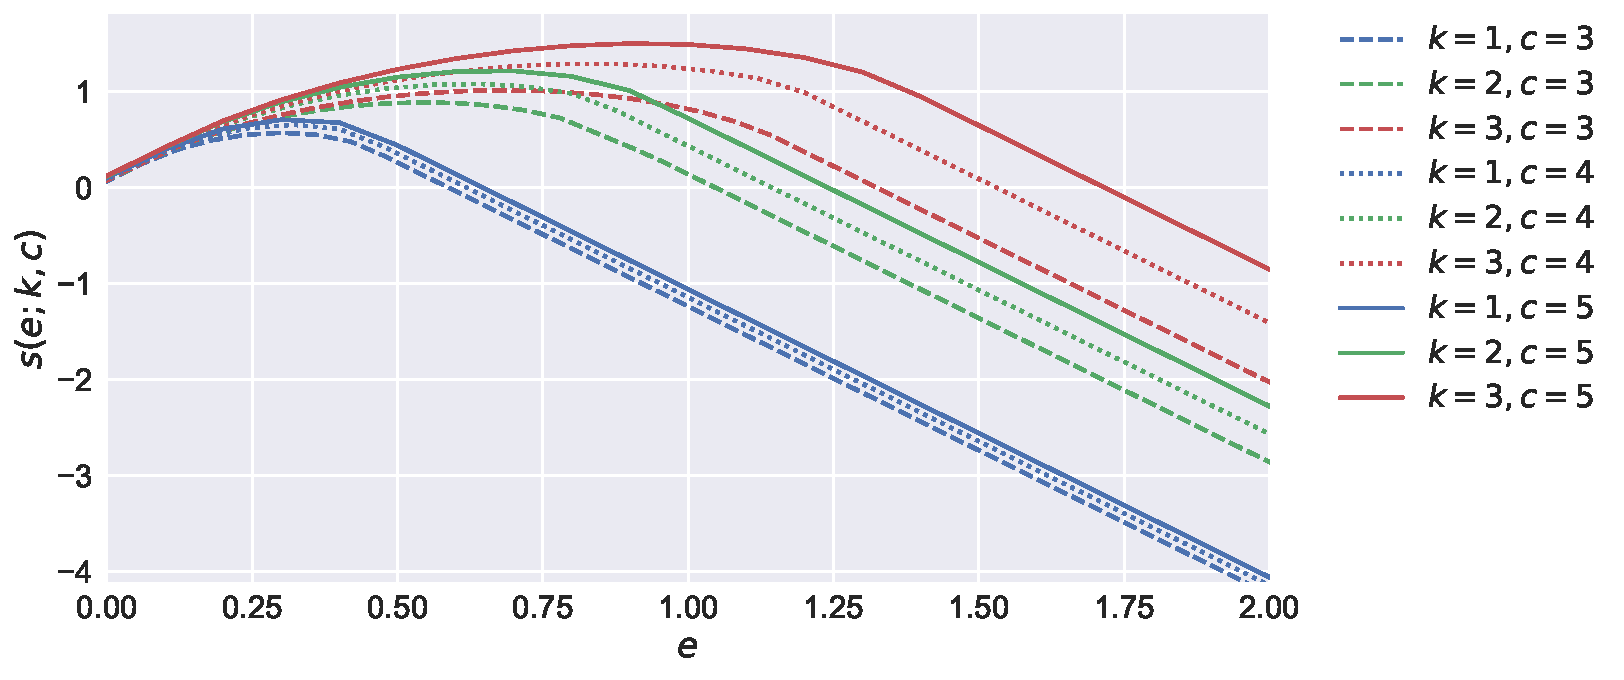
\includegraphics[width=450pt]{hw2/hw2_3(d)}
        \end{figure}
        It can be seen that the result is very similar to the random regular graph in part (c).
        One reasonable explanation is that the self-averaging property and the fact that random $ d $-regular graph ensemble $ \mathbb{G}_{\mathrm{reg}}(N, d) $ and Erd\H{o}s-R\'enyi ensemble $ \mathbb{G}_{\mathrm{ER}}(N, d) $ are asymptotically equivalent when $ N \to \infty $.
        The difference between these two random graph ensemble does not affect the leading exponential order of the partition function.
% \item   
%         Before we start to write the code, we need examine the procedure in part (b) first.
%         We already know how to run BP on a fixed factor graph, but how to run BP on a random graph ensemble?
%         The answer is to use population dynamics (or density evolution): every time we update a BP message, although we do not know how the factor graph looks like, we know the probability distribution of local structure.

%         The distribution of local structure of random graph ensemble is captured by \emph{degree profile} $ (\Lambda, P) $, where
%         \begin{itemize}
%         \item   $ \Lambda(x) = \sum_d \Lambda_d x^d $ is the variable node degree profile
%                 \begin{equation*}
%                     \Lambda_d = \Pr \rdbrs{ \text{a variable node has degree } d}
%                 \end{equation*}
%         \item   $ P(x) = \sum_d P_d x^d $ is the factor node degree profile
%                 \begin{equation*}
%                     P_d = \Pr \rdbrs{ \text{a factor node has degree } d}
%                 \end{equation*}
%         \end{itemize}

%         Let $ \mathsf{ER}_N(c) $ be the ensemble of Erd\H{o}s-R\'enyi random graph ensemble with $ N $ nodes and each edges is present with probability $ p = c / N $.
%         Then in the associated factor graph, each variable node $ (ij) $ has degree $ 2 $, result in $ \Lambda(x) = x^2 $.
%         And each factor node $ i $ has degree $ d $ with probability
%         \begin{IEEEeqnarray*}{rCl}
%             \Lambda_d^{(N)} 
%             &=& \binom{N-1}{d} p^d \rdbrs{ 1 - p }^{N-1-d}
%             = \frac{ \prod_{l=1}^d (N-l) }{ d! } \rdbrs{ \frac{c}{N} }^d \rdbrs{ 1 - \frac{c}{N} }^{N-1-d} \\
%             &=& \frac{c^d}{d!} \sqbrs{ \rdbrs{ 1 - \frac{c}{N} }^{ N/c } }^c \cdot \prod_{l=1}^d \rdbrs{ 1 - \frac{l}{N} } \cdot \rdbrs{ 1 - \frac{c}{N} }^{-(d+1)}
%         \end{IEEEeqnarray*}
%         In the large-$ N $ limit, for finite $ d $, we have
%         \begin{IEEEeqnarray*}{rCl}
%             \Lambda_d
%             &\equiv& \limit{N \to \infty} \Lambda_d^{(N)}
%             = \frac{c^d}{d!} \ee^{-c}, \qquad \forall\, d = 0, 1, \ldots
%             \quad \Rightarrow \quad
%             \Lambda(x) = \ee^{-c} \sum_{d=0}^\infty \frac{c^d}{d!} x^d
%         \end{IEEEeqnarray*}
%         Hence the degree of each factor node is distributed as $ \mathsf{Poisson}(c) $.

%         \begin{algorithm}[H]
%             \begin{center}
%             population dynamics for $ k $-factor problem over ER random graph ensemble
%             \end{center}
%             \KwIn{ensemble parameter $ c $, sample bucket size $ N^{\mathrm{s}} $, iteration $ T $}
%             \KwOut{BP messages after $ T $ BP iteration}
        
%             Initialize $ \clbrs{ \clbrs{ \chi_s^{r, (0)} }_{s \in \mathcal{X}} }_{r=1}^{N^{\mathrm{s}}} $ and $ \clbrs{ \clbrs{ \psi_s^{r, (0)} }_{s \in \mathcal{X}} }_{r=1}^{N^{\mathrm{s}}} $\;
%             \For{$ t = 1, \ldots, T $}{
%                 \For{$ i = 1, \ldots, N^{\mathrm{s}} $} {
%                     Draw $ d $ from $ \mathsf{Possion}(c) $\;
%                     Draw $ j_1, \ldots, j_{d-1} $ uniformly from $ [N^{\mathrm{s}}] $\;
%                     \For{$ s \in \mathcal{X} $} {
%                         Compute $ \tilde{\psi}_s^{i, (t)} = \sum_{ \clbrs{ s_l }_{l=1}^{d-1} } \mathbb{I} \rdbrs{ s + \sum_{l=1}^{d-1} s_l \le k } \prod_{l=1}^{d-1} \chi_{s_l}^{j_l, (t-1)} $\;
%                     }
%                     \For{$ s \in \mathcal{X} $} {
%                         Compute $ \psi_s^{i, (t)} = \tilde{\psi}_s^{i, (t)} \times \sqbrs{ \sum_{s^\prime} \tilde{\psi}_{s^\prime}^{i, (t)} }^{-1} $\;
%                     }
%                 }
%                 \For{$ i = 1, \ldots, N^{\mathrm{s}} $} {
%                     Draw $ j $ uniformly from $ [N^{\mathrm{s}}] $\;
%                     \For{$ s \in \mathcal{X} $} {
%                         Compute $ \tilde{\chi}_s^{i, (t)} = \ee^{\beta s} \psi_s^{j, (t-1)} $\;
%                     }
%                     \For{$ s \in \mathcal{X} $} {
%                         Compute $ \chi_s^{i, (t)} = \tilde{\chi}_s^{i, (t)} \times \sqbrs{ \sum_{s^\prime} \tilde{\chi}_{s^\prime}^{i, (t)} }^{-1} $\;
%                     }
%                 }
%             }
%             \Return $ \clbrs{ \clbrs{ \chi_s^{r, (T)} }_{s \in \mathcal{X}} }_{r=1}^{N^{\mathrm{s}}} $ and $ \clbrs{ \clbrs{ \psi_s^{r, (T)} }_{s \in \mathcal{X}} }_{r=1}^{N^{\mathrm{s}}} $\;
%         \end{algorithm}

%         The next challenge is to compute the expected Bethe free entropy over the entire ensemble.
%         We can treat the output of population dynamics as the empirical distribution of two random probability distribution $ \chi $ and $ \psi $.
%         Since the graph is locally tree-like, all the incoming messages are weakly correlated so that we can assume them to be i.i.d.
%         Then taking average over the whole ensemble, the expected number of edges is $ c N $, hence,
%         \begin{IEEEeqnarray*}{rCl}
%             \limit{N \to \infty} \mathbb{E}_{\mathsf{ER}_N(c)} \sqbrs{ f_{\mathrm{Bethe}}^{k\text{-factor}} }
%             &=& c \, \mathbb{E}_{\psi^{(1)}, \psi^{(2)}} \sqbrs{ \sum_s \ee^{\beta s} \psi_s^{(1)} \psi_s^{(2)} } - 2c \, \mathbb{E}_{\psi, \chi} \sqbrs{ \sum_s \psi_s \chi_s } \\
%             && + \sum_{d=0}^\infty \frac{c^d \ee^{-c}}{d!} \mathbb{E}_{\chi^{(1)}, \ldots, \chi^{(d)}} \sqbrs{ \sum_{\clbrs{ s_l }_{l=1}^d} \mathbb{I} \rdbrs{ \sum_{l=1}^d s_l \le k } \prod_{l=1}^d \chi_{s_l}^{(l)} }
%         \end{IEEEeqnarray*}
%         where the expectations w.r.t. $ \chi $'s and $ \psi $'s can be computed by Monte Carlo.
\end{enumerate}
\end{solution}
\end{document}